%%%%%%%%%%%%%%%%%%%%%%%%%%%%%%%%%%%%%%%%%%%%%%%%%%%%%%%%%%%%%%%%%%%%%%%%%%
% Output voltage u2 for M3C with RLE-Load
%%%%%%%%%%%%%%%%%%%%%%%%%%%%%%%%%%%%%%%%%%%%%%%%%%%%%%%%%%%%%%%%%%%%%%%%%%
\begin{solutionfigure}[htb]
	%   \documentclass{standalone}
	%   \usepackage{pgfplots}
	%   \pgfplotsset{compat=1.18} % Kompatibilität für neuere Versionen
	\centering
	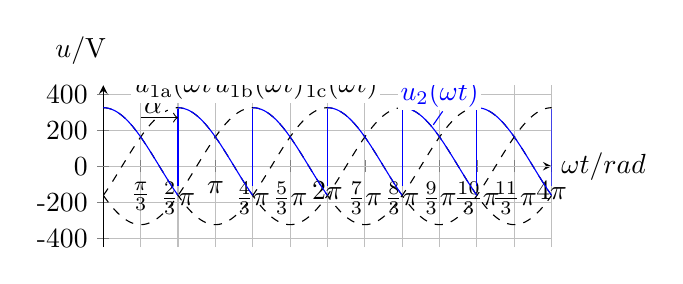
\begin{tikzpicture}
		\begin{axis}[
				% x/y range adjustment
				xmin=0, xmax=720,
				ymin=-450, ymax=450,
				samples=500,
				axis y line=center,
				axis x line=middle,
				extra y ticks=0,
				% Label text
				xlabel={$\omega t / \text{rad}$},,
				ylabel={$u/\mathrm{V}$},
				% Label adjustment
				x label style={at={(axis description cs:1,0.5)},anchor=west},
				y label style={at={(axis description cs:-.05,.97)},anchor=south,yshift=0.2cm},
				width=0.6\textwidth,
				height=0.3\textwidth,
				% x-Ticks
				xtick={0,60,120,180,240,300,360, 420, 480, 540, 600, 660, 720},
				xticklabels={,$\frac{\pi}{3}$,$\frac{2}{3}\pi$,$\pi$, $\frac{4}{3}\pi$,$\frac{5}{3}\pi$,$2\pi$, $\frac{7}{3}\pi$, $\frac{8}{3}\pi$,$\frac{9}{3}\pi$,$\frac{10}{3}\pi$,$\frac{11}{3}\pi$,$4\pi$},
				xticklabel style = {anchor=north},
				% y-Ticks
				ytick={400,200,0,-200,-400},
				yticklabels={400,200,0,-200,-400},
				yticklabel style = {anchor=east},
				% Grid layout
				grid,
				%grid style={line width=.1pt, draw=gray!10},
				%major grid style={line width=.2pt,draw=gray!90},
			]
			% Voltage u1a(wt), u1b(wt) u1c(wt)
			\addplot[black, domain= 0:720,dashed] {325*cos(x)};
			\addplot[black, domain= 0:720,dashed] {325*cos(x+120)};
			\addplot[black, domain= 0:720,dashed] {325*cos(x+240)};

			% Voltage u2(wt)
			\addplot[blue, domain= 0:120] {325*cos(x)};
			\addplot[blue, domain= 120:240] {325*cos(x+240)};
			\addplot[blue, domain= 240:360] {325*cos(x+120)};
			\addplot[blue, domain= 360:480] {325*cos(x)};
			\addplot[blue, domain= 480:600] {325*cos(x+240)};
			\addplot[blue, domain= 600:720] {325*cos(x+120)};
			\addplot[color=blue,solid] coordinates{
					(120,-111)
					(120, 317)
				};
			\addplot[color=blue,solid] coordinates{
					(240,-111)
					(240, 317)
				};
			\addplot[color=blue,solid] coordinates{
					(360,-111)
					(360, 317)
				};
			\addplot[color=blue,solid] coordinates{
					(480,-111)
					(480, 317)
				};
			\addplot[color=blue,solid] coordinates{
					(600,-111)
					(600, 317)
				};
			\addplot[color=blue,solid] coordinates{
					(720,-111)
					(720, 317)
				};
			% Label of u2
			\node[blue, fill=white, inner sep = 1pt, anchor = south] at (axis cs:540,310) {$u_{\mathrm{2}}(\omega t)$};
			% Line to u2
			\draw[thin, blue] (545,305) -- (530,230);
			%Label alpha
			\node[black, fill=white, inner sep = 1pt, anchor = south] at (axis cs:80,275){$\alpha$};
			% Line for alpha
			\draw[->](60,270) -- (120,270);

			% Label of u1c
			\node[black, fill=white, inner sep = 1pt, anchor = south] at (axis cs:370,350) {$u_{\mathrm{1c}}(\omega t)$};
			% Label of u1a
			\node[black, fill=white, inner sep = 1pt, anchor = south] at (axis cs:120,350) {$u_{\mathrm{1a}}(\omega t)$};
			% Label of u1b
			\node[black, fill=white, inner sep = 1pt, anchor = south] at (axis cs:250,350) {$u_{\mathrm{1b}}(\omega t)$};

		\end{axis}
	\end{tikzpicture}
	\caption{Output voltage $u_\mathrm{2}(t)$ for $\alpha = \frac{\pi}{3}$.}
	\label{sfig:subtask3.1_output_voltage}
\end{solutionfigure}